% !TEX root = ../thesis.tex
    
%**************************************************************
% Dataset
%**************************************************************

\chapter{Il dataset di Infostud} \label{cap2}
    Il dataset preso in analisi, relativo a Infostud, gentilmente fornito dal Professor E. Panizzi e dal Dottor 
    E. Bassetti, riveste un'enorme importanza per l'intera comunità accademica de La Sapienza.

    Il dataset rappresenta svariate 
    metriche raccolte dalle piattaforme InfoSapienza e dalle richieste inoltrate attraverso 
    Infostud alla piattaforma esterna GOMP. I dati vengono utilizzati ai fini di monitoraggio e 
    sono raccolti attraverso il software Prometheus. 
    
    \paragraph{Il dataset in dettaglio} La finestra temporale di osservazione dei dati su cui si sono 
    svolti gli studi è lunga poco più di quattro anni, da gennaio 2019 a febbraio 2023, con una frequenza di campionamento di circa 
    una misurazione ogni 15 secondi per le metriche più dense. Il Dottor Bassetti ha anche tenuto traccia di 
    una buona fetta di anomalie effettivamente verificatesi su Infostud nella stessa finestra temporale, 
    garantendo quindi un prezioso ambiente supervised che ha consentito di avere riscontri numerici sulle 
    performance dei modelli in analisi.


    Nel complesso, il dataset è composto da settecentocinquanta file; tali file sono suddivisi per piattaforma, 
    ovvero GOMP e InfoSapienza, e tipologia di metrica. Ciascun file rappresenta 
    circa trenta giorni di osservazioni. Ai fini dell'analisi effettuata con i modelli è stata presa
    in considerazione la parte dei dati strettamente appartenenti a Infostud. 
    
    Di seguito sono riportate in dettaglio le informazioni delle varie tipologie di metriche osservate lato 
    InfoSapienza:
    \begin{enumerate}[leftmargin=14pt]
        \item \texttt{http\_responses}  Contatore di richieste HTTP in cui ogni segnale rappresenta un codice di stato 
                                            riscontrato dalla richiesta. 
                                            Ad esempio, il segnale 200 rappresenta le richieste elaborate con 
                                            successo (codice di stato OK), mentre 401 rappresenta un errore e 
                                            comunica che l'autenticazione HTTP non è riuscita (codice di stato 
                                            Unauthorized). Il contatore è monotonico salvo eventuali reset 
                                            a cadenza non regolare.
        \item \texttt{requests\_total}  Contatore delle richieste totali effettuate a InfoSapienza. Anche qui, il contatore 
                                            è monotonico tra due reset.
        \item \texttt{phoenixws\_requests\_delay\_bucket} 
                                            Ogni segnale rappresenta un bucket a cui è associato un certo valore $le$ (\emph{less or equal}).
                                            Il bucket accumula le latenze delle richieste ai servizi InfoSapienza. 
                                            Ad esempio, se al tempo $t$ avvengono $x$ richieste a $y$ servizi InfoSapienza
                                            e tali richieste vengono risposte con latenza minore o uguale al valore $le$, 
                                            allora tale bucket avrà un valore pari a $x$. È bene 
                                            notare che i bucket non sono disgiunti e il numero di segnali non è uniforme 
                                            tra i file. I segnali, in generale, sono sull'ordine delle centinaia.
        \item \texttt{phoenixws\_requests\_delay\_count}
                                            Contatore di richieste processate a servizi. Ogni segnale è un tipo di servizio
                                            diverso come, ad esempio, la ricerca degli esami o il login. In genere, questi file 
                                            contengono diciotto segnali diversi.
        \item \texttt{phoenixws\_requests\_delay\_sum}
                                            Somma delle latenze delle richieste a servizi. I servizi osservati sono gli 
                                            stessi dei file di tipologia \texttt{phoenixws\_requests\_delay\_count}.                                
    \end{enumerate}

In \hyperref[tab:infosapienza-metrics]{Tabella 2.1.} è illustrato un riassunto delle varie metriche del dataset.
 \begin{table}[H]
    \centering
    \caption{Tipologie di metriche lato Infosapienza.}
    \begin{tabular}{p{0.45\linewidth}p{0.5\linewidth}}
        \toprule
        \textbf{Metrica} & \textbf{Dettagli} \\
        \toprule
        \texttt{http\_responses} & Contatore in cui ogni segnale è associato a un tipo di richiesta HTTP. \\
        \midrule
        \texttt{request\_total} & Contatore totale delle richieste HTTP. \\
        \midrule
        \texttt{phoenixws\_requests\_delay\_bucket} & Insieme di bucket. A ogni bucket è associato un valore $le$ e tale bucket accumula le latenze inferiori o uguali a $le$. \\
        \midrule
        \texttt{phoenixws\_requests\_delay\_count} & Contatore di richieste processate a servizi. Ogni segnale rappresenta un tipo di servizio. \\
        \midrule
        \texttt{phoenixws\_requests\_delay\_sum} & Somma delle latenze delle richieste a servizi. Ogni segnale rappresenta un tipo di servizio. \\
        \bottomrule
    \end{tabular}
    \label{tab:infosapienza-metrics}
\end{table}

    \paragraph{Trasformazione delle etichette}
    Le etichette sono state provvedute sottoforma di file. Ogni file rappresenta 
    un certo intervallo in cui si è verificata un'anomalia. I file hanno anche altre informazioni riportate nella 
    \hyperref[tab:info-labels]{Tabella 2.2}

    Poiché una certa fetta di dataset può contenere più punti all'interno dei vari intervalli di tutti i file delle 
    etichette, è stato creato un dataset binario che mappa un certo timestamp del dataset a un valore di verità: vero 
    se quel timestamp è all'interno di uno degli intervalli dei file delle etichette, ovvero quel timestamp è 
    all'interno di un periodo anomalo del sistema, falso altrimenti.

\begin{table}[H]
    \centering
    \caption{Le informazioni dei file delle etichette.}
    \begin{tabular}{p{0.45\linewidth}p{0.5\linewidth}}
        \toprule
        \textbf{Informazione} & \textbf{Significato} \\
        \toprule
        \texttt{Title} & Tipo di anomalia, ad esempio `Irrangiugibilità Infostud'. \\
        \midrule
        \texttt{Date} & Data di inizio dell'anomalia. \\
        \midrule
        \texttt{resolved} & Valore binario che indica se l'anomalia è stata risolta o no. \\
        \midrule
        \texttt{resolvedWhen} & Data di termine dell'anomalia. \\
        \midrule
        \texttt{Severity} & Grado di severità del problema. \\
        \midrule
        \texttt{affected} & Servizi o insiemi di servizi che hanno subito malfunzionamenti \\
        \bottomrule
    \end{tabular}
    \label{tab:info-labels}
\end{table}

    \paragraph{La scelta del tipo di dataset} \label{cap2:hypothesis} I primi esperimenti si sono basati sui file di tipologia 
    \texttt{http\_responses}. Questi esperimenti non hanno portato a soluzioni di particolare rilievo per 
    ciascun modello applicato, ma sono stati fondamentali per familiarizzare con il dataset. La 
    seconda trance di esperimenti si è focalizzata su tre tipologie di file diversi: 
    \texttt{phoenixws\_requests\_delay\_bucket}, \texttt{phoenixws\_requests\_delay\_count} e 
    \texttt{phoenixws\_requests\_delay\_sum}. È banale che i bucket, essendo la categoria predominante nel 
    dataset, hanno comportato un'elevata esposizione dei modelli a tali dati rispetto che alle altre metriche.
    Difatti gli esperimenti che si sono basati su questi dati non hanno portato soluzioni interessanti. 


    Dopo questi tentativi iniziali, che hanno comunque contribuito a una migliore comprensione dei dati e dei 
    modelli, è stata presa la decisione, in collaborazione con il relatore, il Professore G. Tolomei, di 
    concentrarsi sugli esperimenti successivi utilizzando un dataset ibrido: abbiamo osservato che, 
    avendo a disposizione la somma delle latenze fatte ai servizi di Infosapienza 
    \texttt{phoenixws\_requests\_delay\_sum} e il relativo contatore \texttt{phoenixws\_requests\_delay\_count},
    era possibile creare il dataset che rappresentasse la latenza media di ogni richiesta per ogni servizio. 
    Si prevedeva che questo approccio potesse portare a risultati migliori nell'analisi e nell'individuazione di anomalie.

    
    \paragraph{La scelta della finestra temporale} In virtù delle etichette e del nuovo dataset, dopo un'attenta analisi, 
    gli esperimenti successivi si sono focalizzati su diverse fette temporali che hanno dovuto soddisfare alcune proprietà
    chiave:
    \begin{enumerate}
        \item i dati devono rientrare in una finestra di osservazione all'interno di quella delle etichette, 
              le quali non sono disponibili per tutto il dataset;
        \item la percentuale di anomalie riscontrate deve essere intorno al $5\%$ per garantire al modello di essere addestrato 
              con un numero sufficiente di anomalie, ma non troppe per non rischiare che esso classifichi fluttuazioni anomale 
              come normali;
        \item la suddivisione del dataset in insiemi di training, validazione e test deve garantire a tutti e tre i 
              sottoinsiemi di contenere anomalie ed è auspicabile che la percentuale di anomalie sia quantomeno 
              simile per tutti e tre i sottoinsiemi di dati;
        \item i dati devono essere poco vuoti, ovvero non devono contenere troppi valori nulli per 
              preservare il più possibile l'integrità originale dei dati. Questo perché i modelli, per essere addestrati, 
              necessitano di un dataset privo di valori nulli i quali, purtroppo, sono inevitabilmente presenti;
        \item per limiti computazionali i dati non devono contenere troppi punti, ma al più devono basarsi su tre mesi 
              di osservazioni.
    \end{enumerate}
    
\begin{table}[H]
    \centering
    \caption{Riassunto delle proprietà del dataset su cui verranno basati gli esperimenti.}
    \begin{tabular}{p{0.55\linewidth}p{0.4\linewidth}}
        \toprule
        \textbf{Proprietà} & \textbf{Motivazione}\\
        \toprule
        L'intera finestra temporale delle osservazioni prese in considerazione deve essere inclusa in quella delle 
        etichette. & Consente di avere riscontri numerici sulle performance.  \\
        \midrule
        Percentuale di anomalie $\approx 5\%$. & Le anomalie devono essere presenti e non devono occupare una grande parte di dataset.  \\
        \midrule
        La percentuale di anomalie negli insiemi di training, validation e test deve essere simile e sempre maggiore di zero. 
        & I tre insiemi devono osservare una percentuale simile di anomalie.\\
        \midrule
        I dati non devono contenere molti valori nulli. & Mantiene l'integrità del dataset. \\
        \midrule
        Al massimo tre mesi di osservazioni. & Per soddisfare limiti computazionali.\\
        \bottomrule
    \end{tabular}
    \label{tab:data-properties}
\end{table}

   \paragraph{Pre-processamento dei dati} Per la creazione del dataset delle latenze medie è necessaria una divisione 
   elemento per elemento tra i due dataset \texttt{phoenixws\_requests\_delay\_sum} e \texttt{phoenixws\_requests\_delay\_count}.

   Le proprietà da soddisfare, illustrate nella \hyperref[tab:data-properties]{Tabella 2.3.}, sono varie. Per composizione 
   del dataset, molto problematico è il punto in cui è espressa la necessità che il dataset preso in analisi non debba
   contenere molti valori nulli, e per far sì che venga rispettato è stato doveroso eliminare le righe e le 
   colonne più vuote dei dataset presi in considerazione. 

   I dataset più interessanti che hanno soddisfatto tali proprietà, in seno all'eliminazione delle righe e colonne più 
   vuote, sono tre le cui informazioni sono illustrate nella \hyperref[tab:data-info]{Tabella 2.4.}
    
    \begin{table}[H]
        \centering
        \caption{Statistiche del dataset suddiviso in finestre temporali.}
        \begin{tabular}{lccc}
            \toprule
            \textbf{Finestra temporale} & \textbf{Anomalie (\%)} & \textbf{Valori nulli (\%)}  \\
            \toprule
            8 agosto - 11 novembre 2019  & 6\%   & 15\% \\
            23 febbraio - 24 marzo 2020  & 2.1\% & 16\%  \\
            23 maggio - 22 giugno 2020   & 5.6\% & 14.5\%  \\
            \bottomrule
        \end{tabular}
        \label{tab:data-info}
    \end{table}

    Tali porzioni di dataset, purtroppo, come illustrato, ancora presentano valori nulli. Per poter permettere ai modelli
    di essere applicati, è necessario sostituire i valori nulli con un valore che si presti bene al problema. In questi studi,
    i valori nulli sono stati sostituiti con la media relativa a ogni segnale. 

    Gli esperimenti sono stati condotti principalmente utilizzando il dataset relativo 
    al periodo dal 23 maggio al 22 giugno 2020, ma tutti i modelli possono essere applicati in maniera analoga a tutti 
    i dataset menzionati, con l'adeguamento degli iperparametri. 
    
    Il dataset preso in analisi ha visto la rimozione di un circa un quarto delle righe e un terzo delle 
    colonne meno dense, da diciotto a dodici.

    \begin{figure}[H]
        \centering
        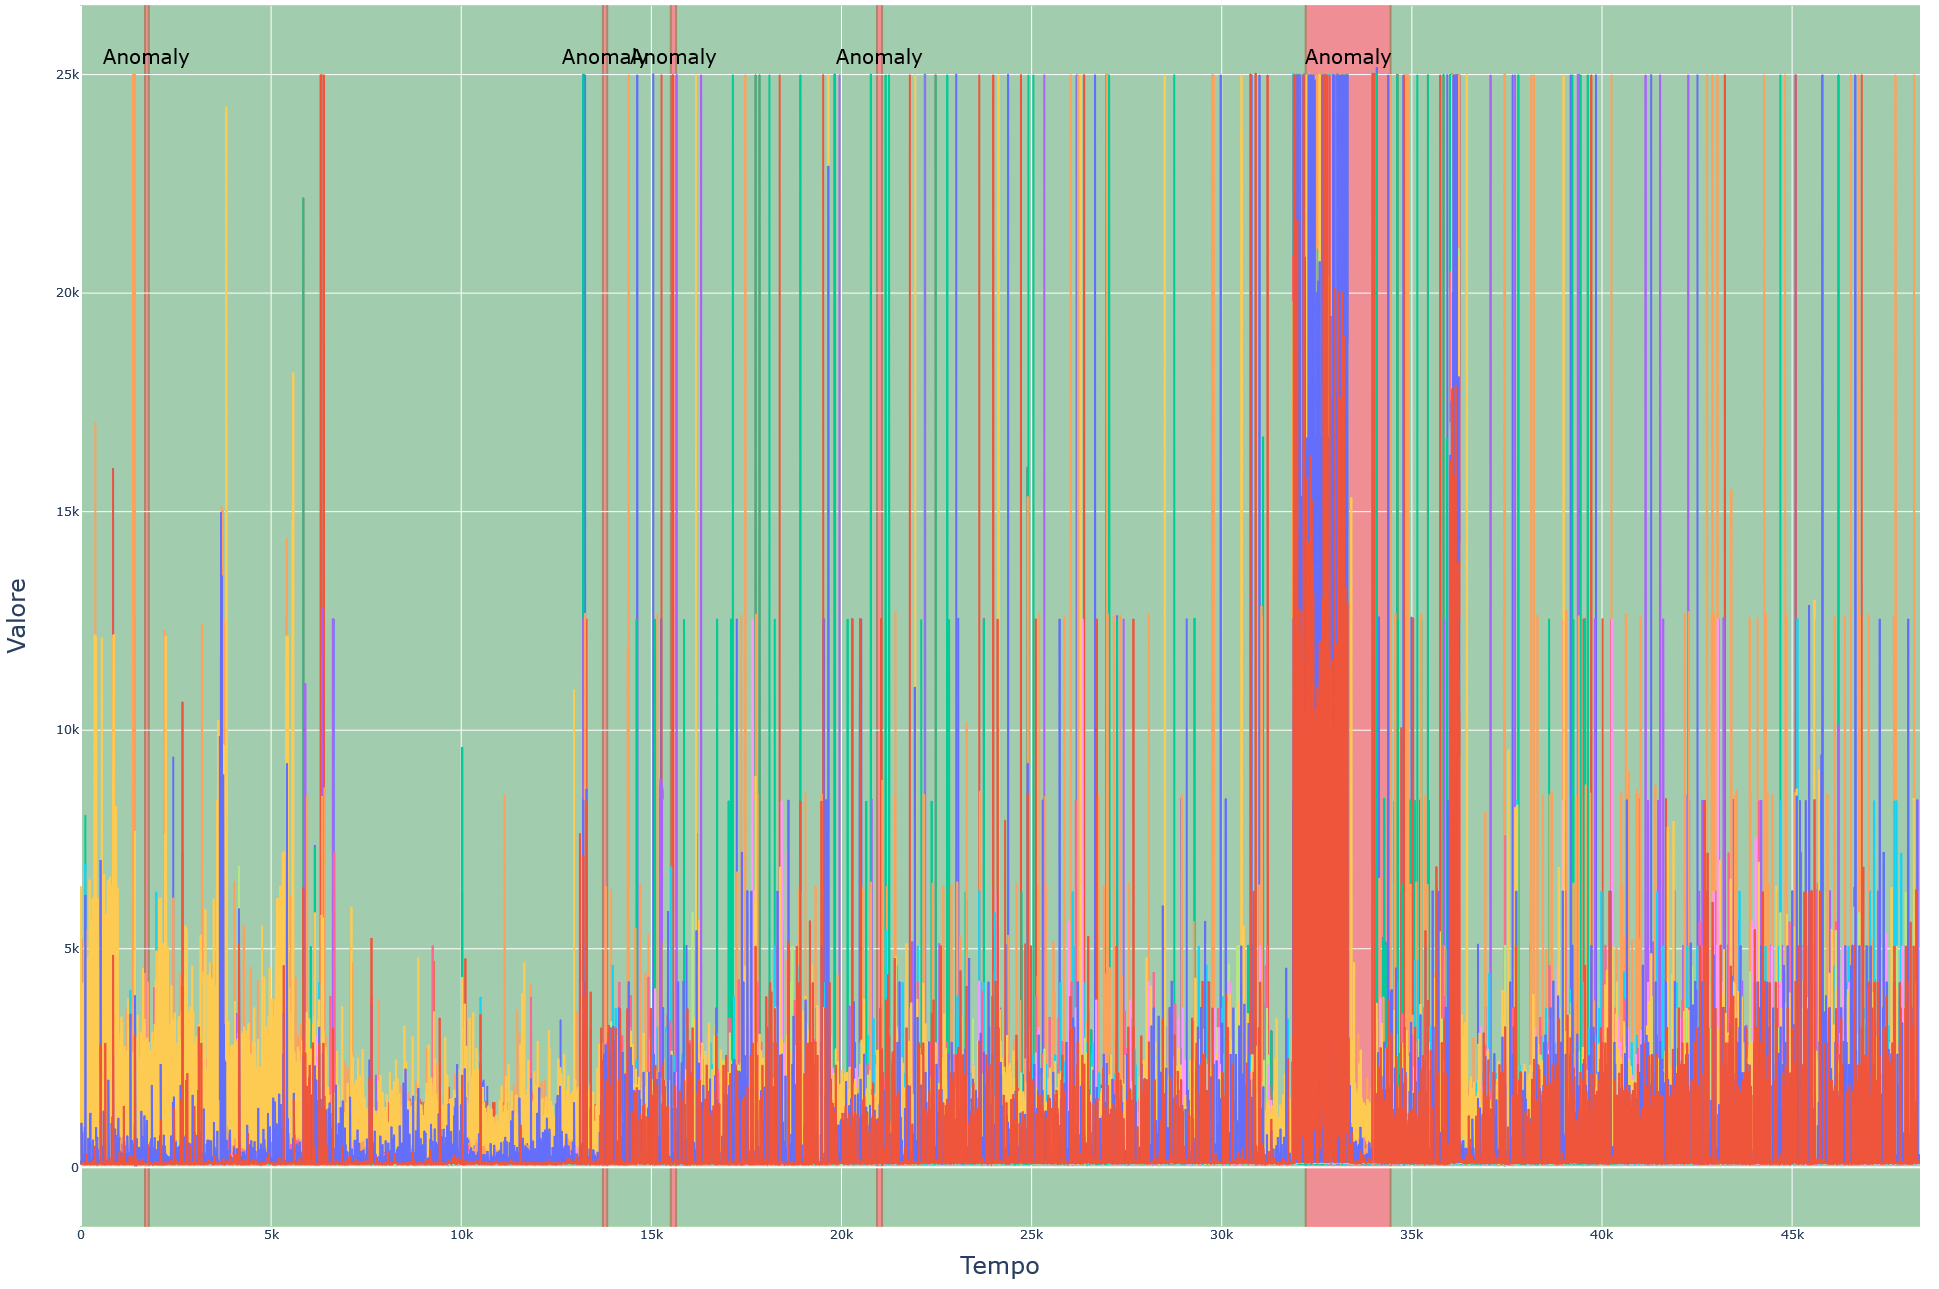
\includegraphics[width=0.6\textwidth]{./input/chapters/figs/plot-infostud.png}
        \caption{Dataset 23 maggio - 22 giugno 2020. Le bande rosse rappresentano le anomalie ground-truth, mentre quelle 
        verdi i periodi non anomali.}
        \label{fig:dataset-giugno}
    \end{figure}
    \begin{figure}[H]
        \centering
        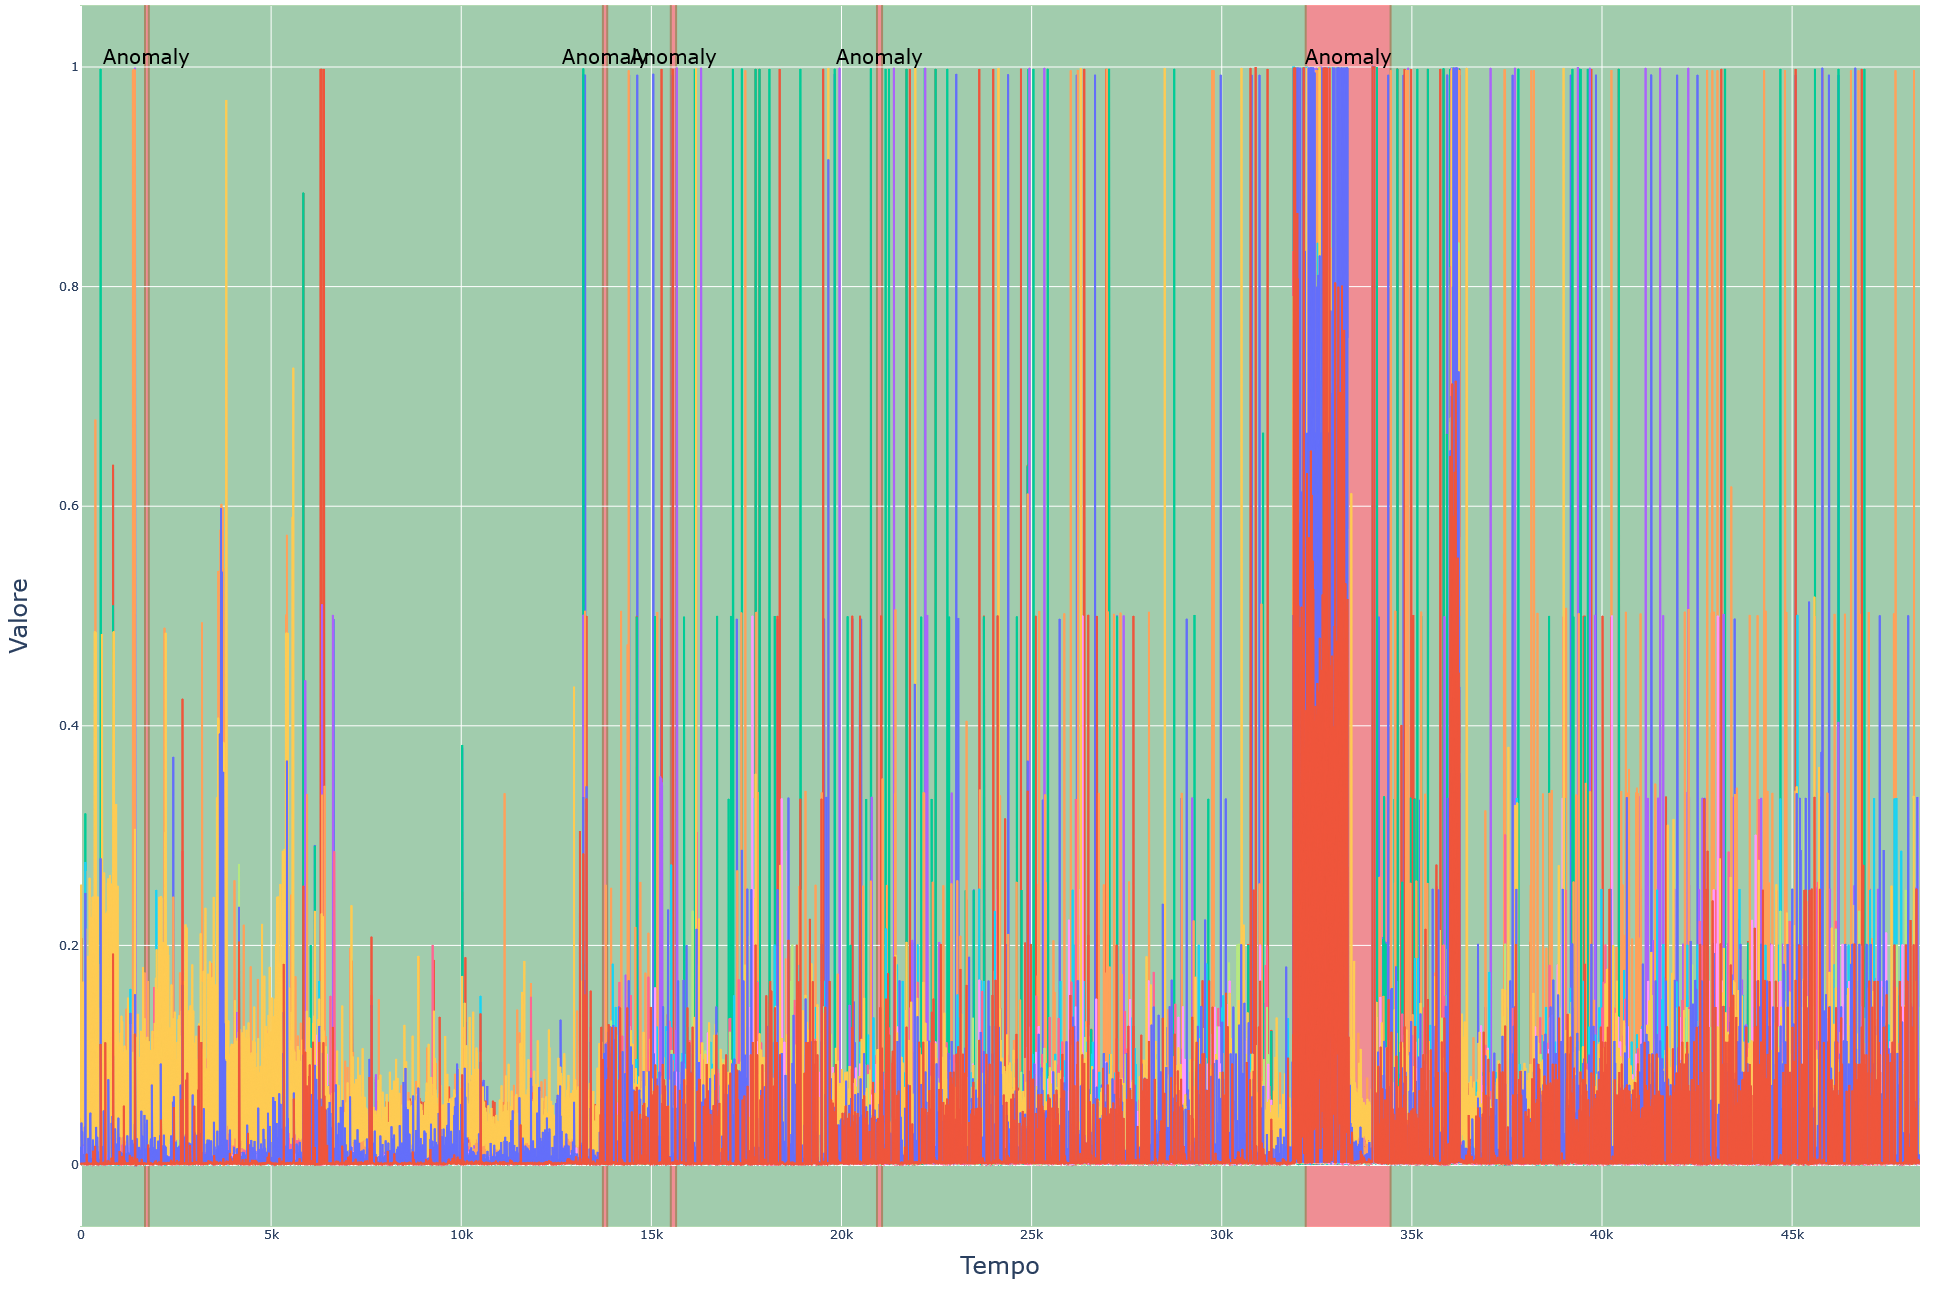
\includegraphics[width=0.6\textwidth]{./input/chapters/figs/plot-infostud-norm.png}
        \caption{Dataset 23 maggio - 22 giugno 2020 normalizzato senza valori vuoti. Le bande rosse rappresentano le anomalie ground-truth, mentre quelle 
        verdi i periodi non anomali.}
        \label{fig:dataset-giugno-norm}
    \end{figure}    
    

\paragraph{Visualizzazione del dataset preso in analisi}
    Il dataset su cui si basano gli esperimenti dei capitoli successivi è illustrato in 
    \hyperref[fig:dataset-giugno]{Figura 2.1.} 
    
    Possiamo osservare le anomalie che si sono presentate nelle aree in cui lo sfondo del grafico è rosso, 
    mentre le aree verdi rappresentano i periodi non anomali. È lampante che, nell'ultima anomalia, quella più 
    grande tra tutte le altre, i segnali sono molto più alti. Ci aspettiamo che un modello segnali quei periodi come 
    anomali. In \hyperref[fig:dataset-giugno-norm]{Figura 2.2.} possiamo osservare il dataset normalizzato con i 
    valori vuoti sostituiti dalla media relativa al segnale associato.

    È un privilegio poter affermare che l'applicazione di modelli metodologicamente diversi sul dataset di Infostud, indispensabile
    per la comunità Sapienza, rappresenta una straordinaria opportunità per gli studi intrapresi dal sottoscritto.